% !TeX spellcheck = es_AR
\documentclass[a4paper,spanish,12pt,twoside]{article}
\usepackage{geometry}
\geometry{
	a4paper,
	total={170mm,257mm},
	left=20mm,
	top=20mm,
}
\usepackage[utf8]{inputenc}
\usepackage[spanish]{babel}
\usepackage{graphicx}
\graphicspath{ {imagenes/} }
\usepackage{amsmath}
\usepackage{graphicx}
\usepackage{wrapfig}
\usepackage{parskip}
\usepackage{listings}
\usepackage[obeyspaces]{url}
\usepackage{caption}
\usepackage{subcaption}
\captionsetup[figure]{name={Figura},labelsep=period}
%\captionsetup[table]{name={Tabla}}
\usepackage{multirow}
\usepackage{textcomp} % ° symbol
\usepackage{amsmath}
\usepackage{float} %
\usepackage[hidelinks]{hyperref}


\title{Trabajo final de Computación paralela: \textit{tiny md}}
% \footnote no funciona con \maketitle => \thanks
\author{Francisco Fernández}
\date{\today}

\begin{document}

\maketitle

\

\

\begin{abstract}

AGREGAR RESUMEN CUANDO TERMINE\footnote{Directorio de GitHub: \url{https://github.com/fernandezfran/tiny_md}}%


\end{abstract}

%\end{titlepage}

\section{Introducción teórica al problema}

La dinámica molecular (MD, de sus siglas en inglés, Molecular Dynamics) es una técnica de simulación computacional que considera la interacción entre partículas atómicas para obtener una evolución temporal de las mismas. Esto se logra resolviendo numéricamente las ecuaciones de movimiento de Newton. A partir de cantidades microscópicas (posiciones ($x$), velocidades ($v$), fuerzas ($f$)) se pueden obtener propiedades termodinámicas macroscópicas del sistema en equilibrio (temperatura ($T$), presión ($P$)). Esta técnica tiene aplicaciones en muchas áreas del conocimiento, tales como física, química, biofísica, ciencias de los materiales, etc.

\subsection{Programa de MD}

Una descripción simple de un programa de dinámica molecular se introduce a continuación:

\begin{itemize}
 \item \textit{Inicialización del sistema}: se especifican la cantidad de partículas $N$, la temperatura de referencia $T$ y la densidad $\rho$, de donde puede obtenerse el volumen $V$, largo de la caja $L$. Además, se elije $r_{cut}$, el paso temporal $dt$, las posiciones y velocidades iniciales.
 \item \textit{Cálculo de fuerzas}: se computan las fuerzas de todas las partículas.
 \item \textit{Integración de las ecuaciones de movimiento}: se integran las ecuaciones de Newton, con algún integrador que a partir de la condición anterior obtiene las posiciones y velocidades del paso temporal siguiente.
 \item \textit{Mediciones}: se realizan cálculos de distintas cantidades de interés (energía potencial, cinética, presión, temperatura).
 \item \textit{Evolución temporal}: $t = t + dt$.
\end{itemize}

A continuación se amplia cada una de estas secciones específicamente para el programa presentado. Ya que hay distintas formas de inicializar el sistema, de calcular las fuerzas con distintos potenciales, algoritmos de evolución, etc.

\subsubsection{Inicialización del sistema}

En este caso las posiciones se inicializan dentro de una red cristalina $FCC$ y las velocidades se dan aleatoriamente entre $-0.5$ y $0.5$, se les resta la velocidad del centro de masa para que el sistema no se esté desplazando y se las multiplica por un factor que involucra la temperatura.


\subsubsection{Condiciones periódicas de contorno e imagen mínima}

En el caso simulado acá se utilizan condiciones periódicas de contorno (pbc, periodic boundary conditions), las mismas buscan reproducir un sistema infinito para que no haya efectos de borde y consisten en considerar las $N$ partículas como una celda primitiva de una red infinita de celdas idénticas, en donde, si una partícula sale por un extremo de la caja, ingresa por el opuesto.

\begin{figure}[h]
	\centering
	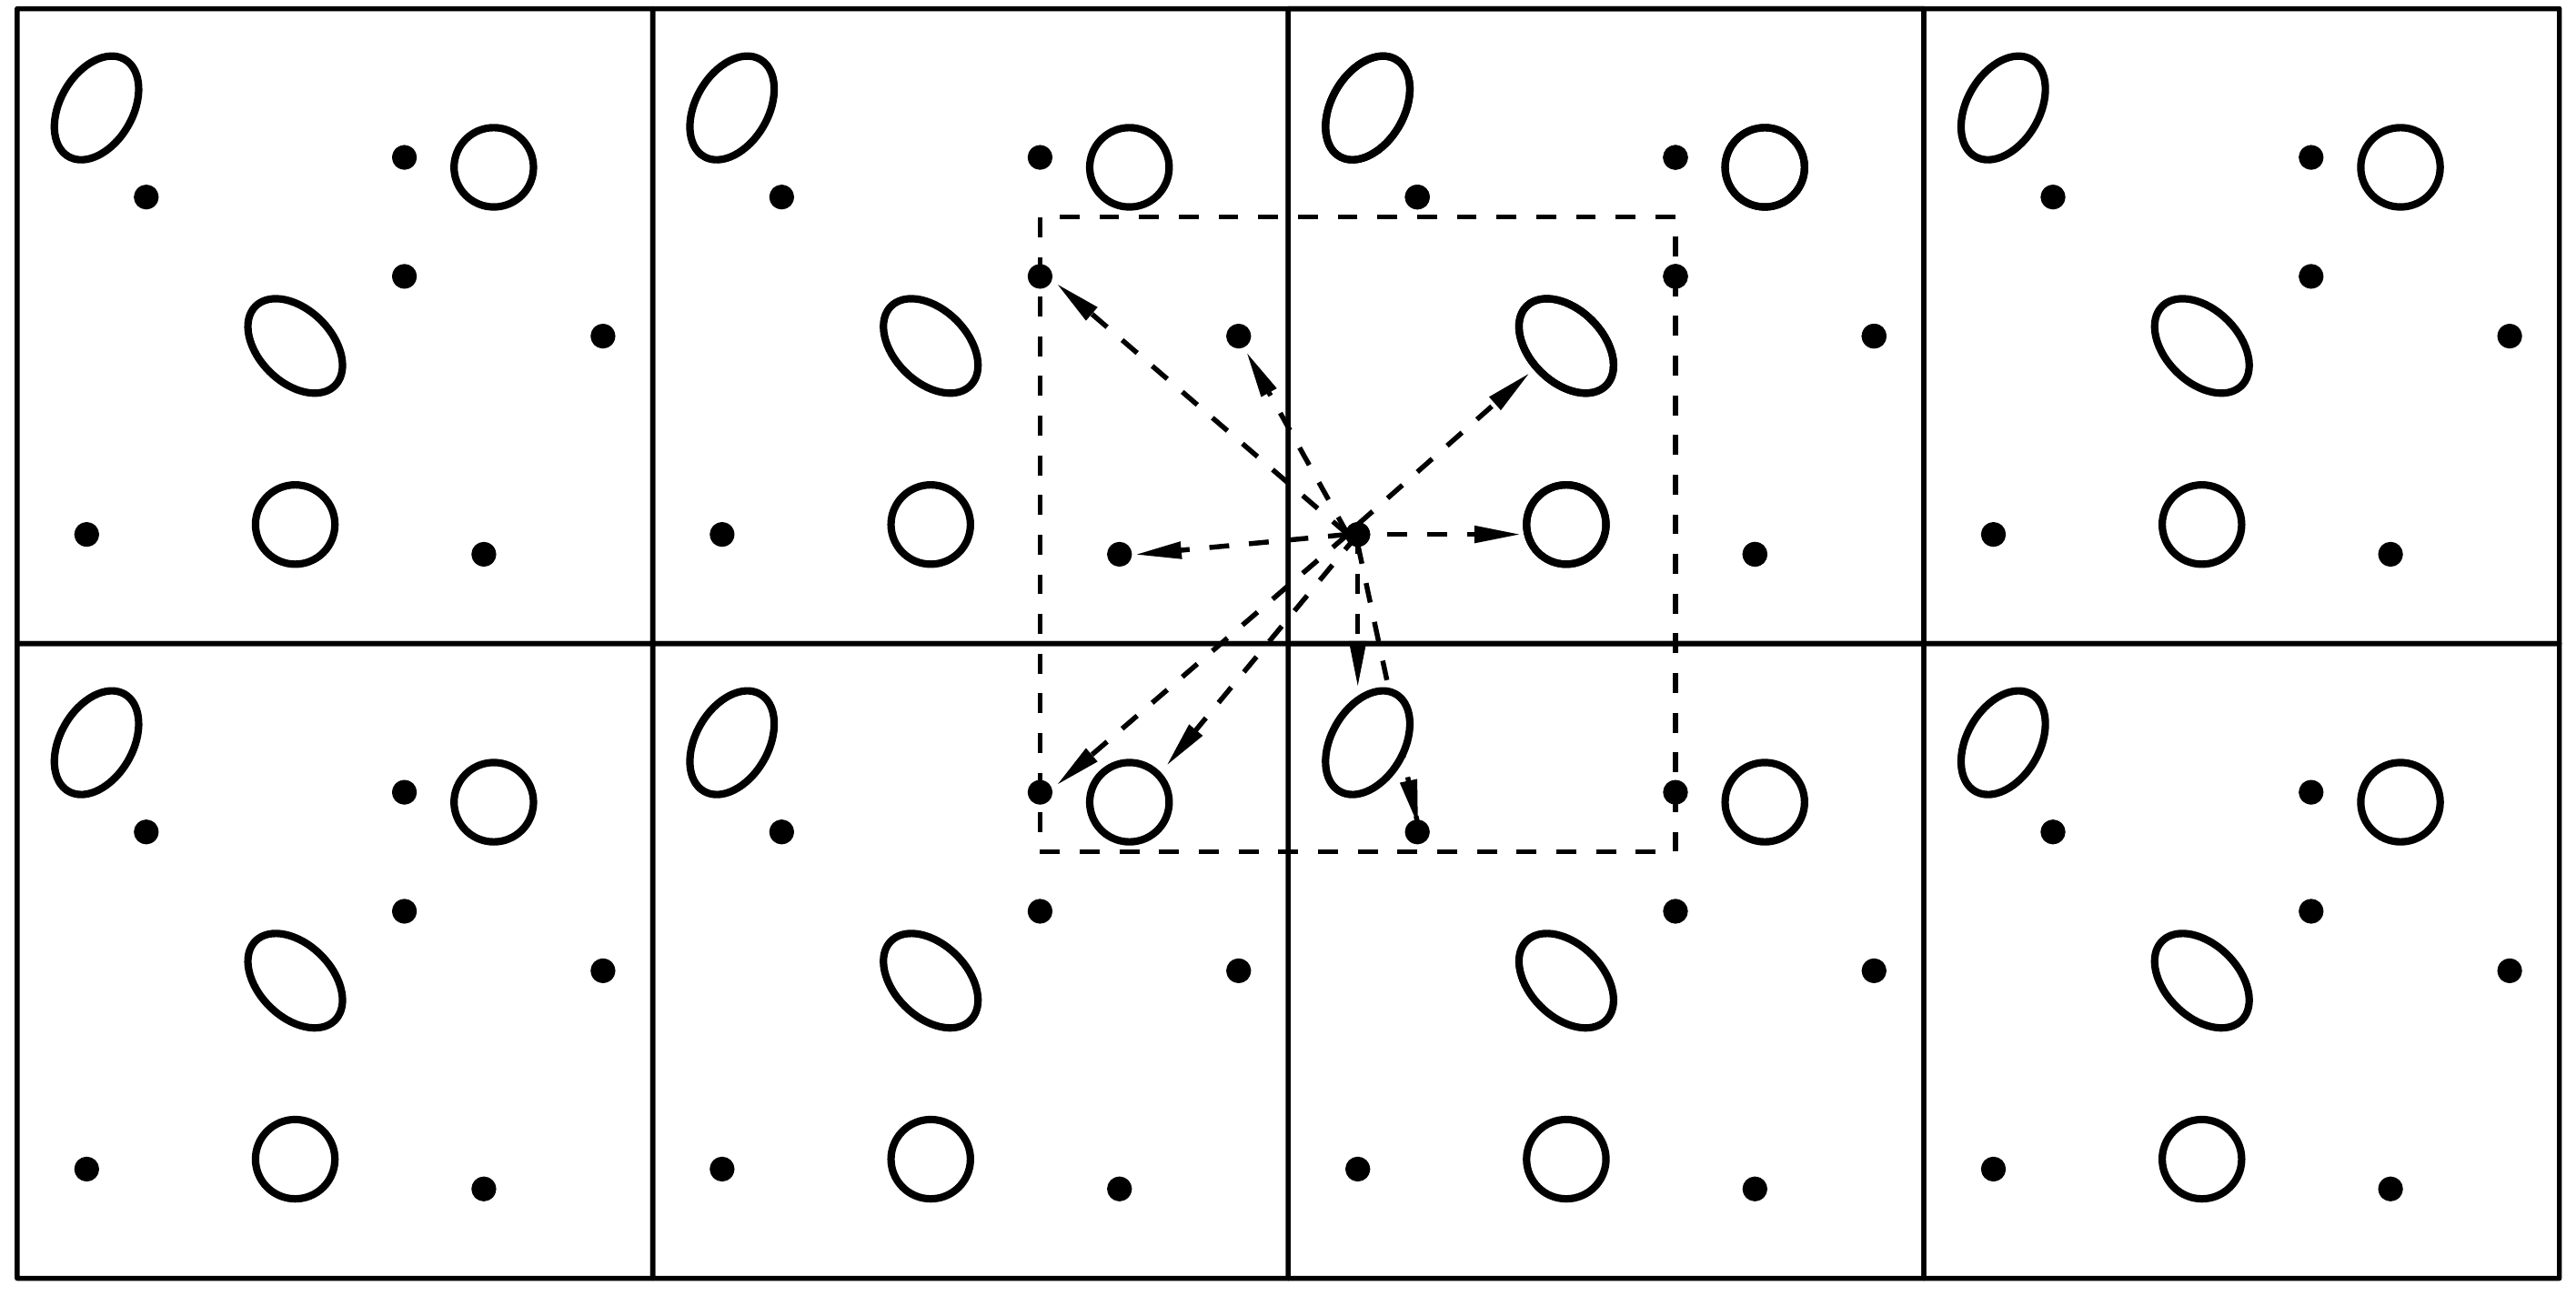
\includegraphics[width=.7\textwidth]{pbc.png}
	\caption{Condiciones periódicas de contorno e imagen mínima.}
	\label{fig:pbc}
\end{figure}

En la figura \ref{fig:pbc} puede verse como se replica una misma celda en todas las direcciones y como al estar centrado en una partícula es necesario salirse de la celda hacia celdas vecinas para encontrar la imagen mínima, que es la distancia más cercana a una partícula.

\subsubsection{Cálculo de fuerzas}

Para el cálculo de las fuerzas se utiliza un potencial aditivo de a pares de Lennard--Jones (12--6), dado por la siguiente expresión,
$$
V_{LJ}(r) = 4\varepsilon \left[ \left( \frac{\sigma}{r} \right)^{12} - \left( \frac{\sigma}{r} \right)^6 \right],
$$
donde $r$ es la distancia entre dos partículas, $\sigma$ es el ``tamaño de la partícula'' y $\varepsilon$ indica que tan profundo es el potencial en el mínimo $r_m = 2^{1/6}\sigma$. La forma funcional se muestra en la figura \ref{fig:lj}, si la distancia entre dos pares de partículas es menor a $r_m$ se repelen, si la distancia es mayor, se atraen, y no interactúan si la distancia es infinita.

Antes de calcular las fuerzas, se necesita la distancia entre dos partículas $i$ y $j$, utilizando la regla de la imagen mínima para considerar la distancia a la imagen más cercana, y calculando la fuerza sólo si dicha distancia es menor a un radio de corte, $r_{cut}$, de la siguiente forma
$$
f_x(r) = -\frac{\partial u(r)}{\partial x} = - \left(\frac{x}{r}\right) \left( \frac{\partial u(r)}{\partial r} \right),
$$
que para el caso del potencial de Lennard--Jones queda
$$
f_x(r) = \frac{24x}{r^2} \left( \frac{2}{r^{12}} - \frac{1}{r^6} \right)
$$
tanto para $x$ como para $y$ y $z$.

\begin{figure}[h]
	\centering
	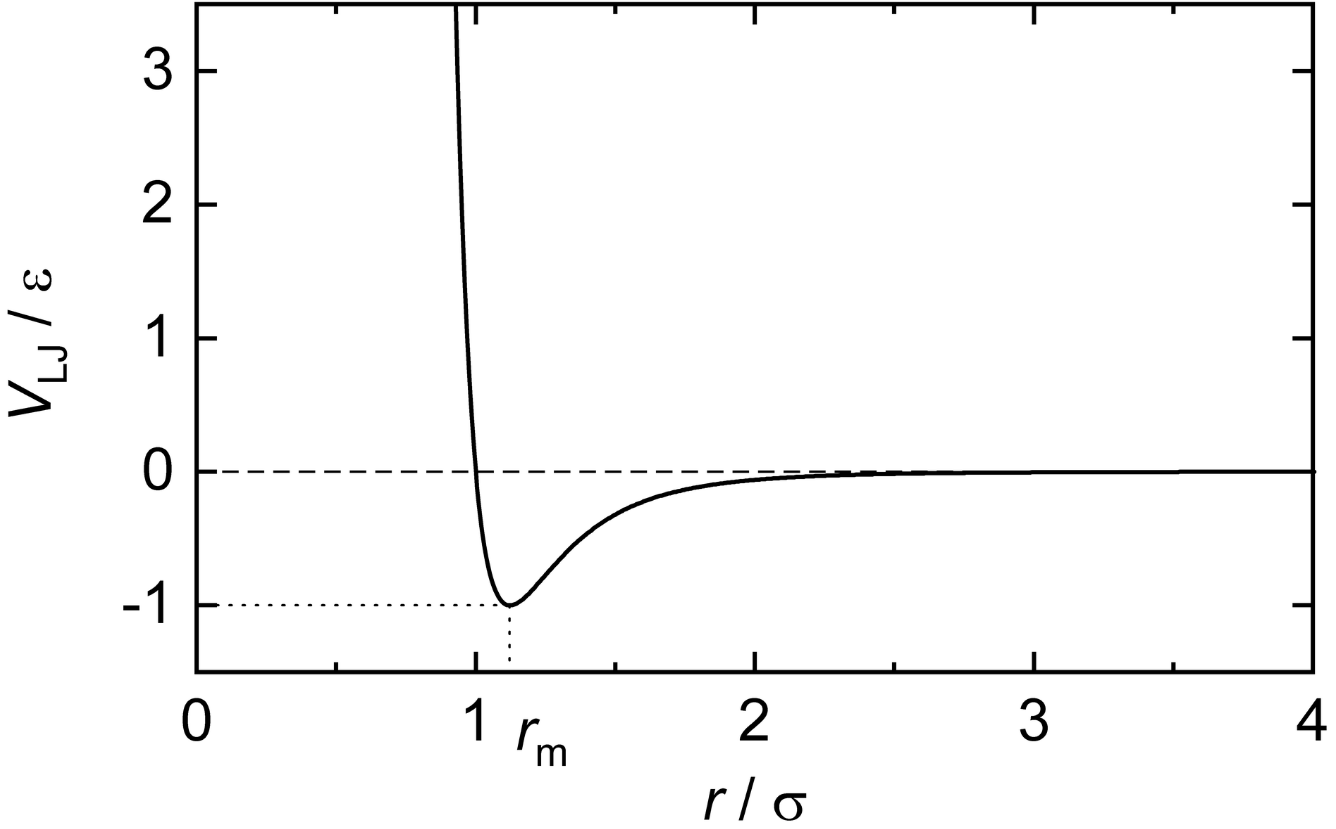
\includegraphics[width=.7\textwidth]{lj.png}
	\caption{Gráfico del potencial de Lennard--Jones.}
	\label{fig:lj}
\end{figure}

Dentro de esta misma sección de código se calcula la energía potencial y la presión instantáneas. 

\subsubsection{Integración de las ecuaciones de movimiento}

Se utiliza el algoritmo \textit{Velocity Verlet}, el mismo conserva la energía total del sistema si se encuentra en el ensamble NVE, que para las posiciones se ve como un desarrollo de Taylor,
$$
r(t + \Delta t) = r(t) + v(t) \Delta t + \frac{f(t)}{2m} \Delta t^2,
$$
y a las velocidades se las actualiza como
$$
v(t + \Delta t) = v(t) + \frac{f(t + \Delta t) + f(t)}{2m} \Delta t,
$$
esto exige calcular las velocidades una vez que se obtuvieron las nuevas posiciones y, a partir de ellas, las nuevas fuerzas.

Aquí se calcula la energía cinética y la temperatura instantáneas.

\subsubsection{Mediciones}

Tanto a la energía potencial como a la presión es necesario sumarles una contribución de cola debido al \textit{truncado y desplazado} que se realiza en $r_{cut}$, para que el potencial se anule en este punto, esto asumiendo que la energía potencial aportada por una partícula es dominada por las interacciones de las partículas más cercanas. Para la presión se tiene
$$
P_{tail} = \frac{16}{3}\pi\rho^2\varepsilon\sigma^3 \left[ \frac{2}{3}\left( \frac{\sigma}{r} \right)^9 - \left( \frac{\sigma}{r} \right)^3 \right],
$$
y para la energía
$$
U_{tail} = \frac{16}{3}N\pi\rho\varepsilon\sigma^3 \left[ \frac{2}{3}\left( \frac{\sigma}{r} \right)^9 - \left( \frac{\sigma}{r} \right)^3 \right].
$$

La presión total será una suma de esta contribución de cola y la presión del virial
$$
P = \rho k_BT + \frac{1}{dV} \left\langle \sum_{i<j} \mathbf{f}(\mathbf{r}_{ij}) \cdot \mathbf{r}_{ij} \right\rangle,
$$
donde $k_B$ es la constante de Boltzmann y $d$ la dimensión del sistema.

La energía total es la suma de la contribución de cola más la suma que se obtiene a través de la interacción entre las partículas a través del potencial de Lennard--Jones.

Por otro lado, tanto la energía cinética como la temperatura se obtienen utilizando las velocidades de la siguiente manera
$$
E_{kin} = \frac{1}{2} \sum_{i=1}^N m_i v_i^2,
$$
$$
k_BT = \frac{1}{3N} \sum_{i=1}^{N} m_i v_i^2
$$
donde $m_i$ es la masa de la partícula $i$

\subsection{Ecuación de estado}

La ecuación de estado relaciona las variables de un sistema bajo ciertas condiciones físicas. En este caso se presenta la presión en función de la densidad del sistema, es decir, se realizan simulaciones en el ensamble canónico (NVT) en las que inicialmente se fija un volumen y la temperatura se mantiene reescaleando las velocidades, para cada una de ellas se calcula la presión para obtener la ecuación de estado $P$ vs $\rho$ que se muestra en la figura \ref{fig:eos}. Para densidades altas el sistema se comporta como un sólido, las posiciones iniciales del cristal FCC se mantienen, y para densidades bajas se comporta como un líquido en el cual las partículas están desorganizadas.

\begin{figure}[h]
	\centering
	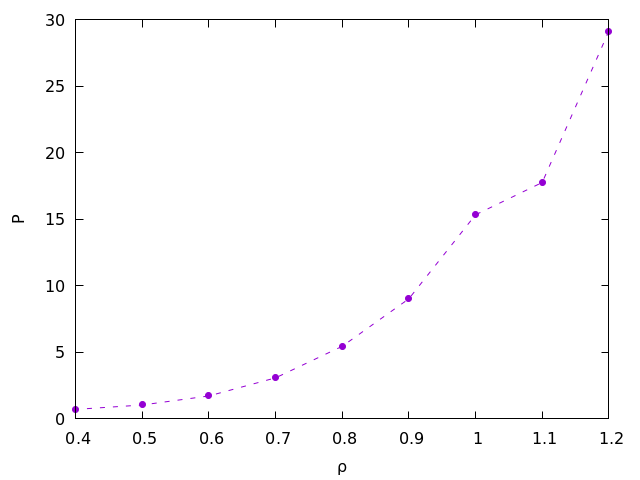
\includegraphics[width=.7\textwidth]{eos.png}
	\caption{Ecuación de estado para la isoterma $T=2.0$.}
	\label{fig:eos}
\end{figure}


\section{Resultados y discusiones}

\subsection*{Unidades y métrica}

Las unidades en las que se encuentran las cantidades físicas dentro del programa son unidades reducidas de Lennard--Jones. Esto quiere decir que se considera $k_B = 1$, que la masa está medida en unidades de $m$, que la distancia está medida en unidades de $\sigma$ y la energía en unidades de $\varepsilon$. A partir de esto se pueden convertir los valores de todas las propiedades físicas, por ejemplo, $T^* = k_BT/\varepsilon$ y $t^* = t \sqrt{\varepsilon/m\sigma^2}$, donde $*$ como superíndice quiere decir que es la forma reducida.

Una métrica usual de dinámica molecular es $ns/day$, es decir, cuántos nanosegundos evoluciona el sistema en un día de simulación. Esta métrica está implementada en el código pero depende del tamaño del problema. En algunas gráficos se presenta la misma y en otras el tiempo total de simulación.

\subsection*{perf}

En la figura \ref{fig:perf-report} se muestra lo obtenido al realizar \path{perf record ./tiny_md && perf report}. Más del 95\% del tiempo se computo se consume en las funciones \path{forces} y \path{pbc} (que es llamaba por \path{forces} y \path{velocity_verlet}), así que estas son las secciones de código en las que se necesitan hacer optimizaciones.
\begin{figure}[h]
	\centering
	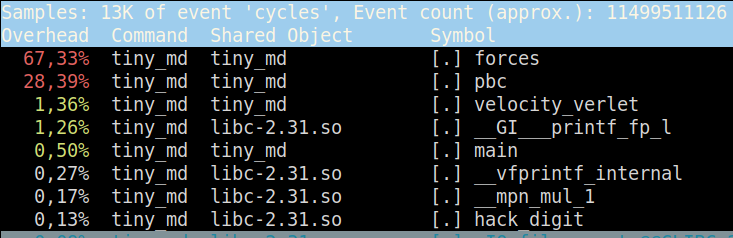
\includegraphics[width=.7\textwidth]{perf-report.png}
	\caption{Porcentaje del tiempo simulado en las funciones del código.}
	\label{fig:perf-report}
\end{figure}

\subsection{Optimizaciones secuenciales}

\subsection{Vectorización}

\subsection{OpenMP}

\end{document}